\documentclass[12pt]{gshs_lecture}

\usepackage{datetime}
\usepackage{framed}
\usepackage{verbatim}
\usepackage{color}
\usepackage{ulem}
\usepackage{amsmath,amssymb}
\usepackage{graphicx}
\usepackage{booktabs}
\usepackage{fancyvrb}
\usepackage{hyperref}
\usepackage{subfigure}
\usepackage{pdfpages}
\usepackage{setspace}
\usepackage{listings}
\usepackage{tikz}
\usepackage{siunitx}
\usepackage{listings}
\usepackage{pgfplots}

\lstset{basicstyle=\scriptsize, tabsize=4, numbers=left, keywordstyle=\color{magenta}, commentstyle=\color{green}}

\makeatletter
\newcommand*{\rom}[1]{\expandafter\@slowromancap\romannumeral #1@}
\makeatother

\newdate{date}{16}{10}{2019}

%% Title, Author, Institute, Date %%
\title[]{2019 \LaTeX\ 워크샵}
\subtitle[]{latex.gs.hs.kr}
\author[]{경기과학고 \TeX\ 사용자협회 35기}
\institute[GSHS]{Gyeonggi Science High School\\ for the gifted}
\date[]{\displaydate{date}}

\setbeamertemplate{caption}[numbered]
\renewcommand{\baselinestretch}{1.25}

\newcommand{\tb}{\textbackslash}
\newcommand{\comb}[2]{{}_#1C_#2}
\newcommand{\gs}{Gyeonggi Science High School }

\newenvironment{codeblock}[1]{
	\begin{block}{#1}
		\setstretch{1.0}
		\begin{small}
}{
		\end{small}
	\end{block}
}

\begin{document}

\begin{frame}[plain]
\titlepage
\end{frame}
\setbeamertemplate{sidebar left}[sidebar theme]

\begin{frame}[t]{Outline}
\tableofcontents%[currentsection]
\end{frame}


\section{General Tips}

\begin{frame}[t]{자동 조사 기능}
	\begin{itemize}
		\item 그림 삽입시 '그림 1을 보면', '그림 2를 보면'...
		\item '1','2' 는 \texttt{\tb ref\{\}}를 사용하면 된다.
		\item 하지만 조사는?
		\item 매번 바꿔줘야 할까?
		\item \LaTeX 에는 자동 조사 기능이 있다.
	\end{itemize}
	
	\begin{codeblock}{자동 조사 기능}
		\tb 이, \tb 가, \tb 을, \tb 를, \tb 와, \tb 과, \tb 로, \tb 으로, \tb 은, \tb 는, \tb 라, \tb 이라 \\
		그림 \texttt{\tb ref\{...\} \tb 을 보면...}
	\end{codeblock}
\end{frame}

\begin{frame}[t]{사용자 지정 명령어}
	\begin{itemize}
		\item 논문을 쓰면서 자주 써야 하는 문구, 수식 등이 있는데 이를 매번 타이핑 해야 할까?
		\item 프로그래밍 언어에서의 함수처럼 코드를 작성할 수는 없을까?
		\item \texttt{\tb newcommand\{\}}를 사용하자
		\item \texttt{\tb newcommand\{명령어 이름\}\{정의\}}
		\item \texttt{\tb newcommand\{명령어 이름\}[인자 개수]\{정의\}}
	\end{itemize}
	
	\begin{codeblock}{사용자 지정 명령어}
		\texttt{\tb newcommand\{\tb gs\}\{Gyeonggi Science High School \}}\\
		\texttt{\tb newcommand\{\tb comb\}[2]\{\{\}\_\#1C\_\#2\}}
	\end{codeblock}
\end{frame}

\begin{frame}[t]{사용자 지정 명령어}
	\begin{center}
		Gyeonggi Science High School is the first.\\
		Gyeonggi Science High School is the best. \\
	\end{center}
	
	\begin{center}
		${}_{4}C_{2}=6$
	\end{center}
	
	\begin{codeblock}{사용자 지정 명령어}
		\texttt{\tb newcommand\{\tb gs\}\{Gyeonggi Science High School \}}\\
		\texttt{\tb gs is the first.\tb\tb \\
			\tb gs is the best.} \\
		
		\texttt{\tb newcommand\{\tb comb\}[2]\{\{\}\_\#1C\_\#2\}}\\
		\texttt{\$\tb comb\{4\}\{2\}=6\$}
	\end{codeblock}
\end{frame}

\begin{frame}[t]{siunitx}
	\begin{itemize}
		\item SI unit을 나타낼 때 편한 package
		\item \texttt{\tb usepackage\{siunitx\}}
	\end{itemize}
	
	\begin{center}
		\ang{45},\ \ \ang{60;10;54}\\
		\num{1.5e15}\\
		\si{\kilo\meter},\ \ \si{\kilogram\meter\per\second\squared}\\
		\SI{1.6e-19}{\coulomb}
	\end{center}
	
	\begin{codeblock}{siunitx}
		\texttt{\tb ang\{45\}, \tb ang\{60;10;54\}\\
			\tb num\{1.5e15\}\\
			\tb si\{\tb kilo\tb meter\}, \tb si\{\tb kilogram\tb meter\tb per\tb second\tb squared\}\\
			\tb SI\{1.6e-19\}\{\tb coulomb\}}
	\end{codeblock}
\end{frame}

\begin{frame}[t,fragile]{코드 삽입}
	\begin{itemize}
		\item Appendix에 코드를 삽입할 때는 어떻게 해야 할까?
		\item \texttt{\tb usepackage\{listings\}}
	\end{itemize}
	
	\begin{center}
	\begin{tabular}{c}
		\begin{lstlisting}[language = c++]
#include<cstdio>

int f(int x)
{
	return x + 1;
}

int main()
{
	int n;
	scanf("%d", &n);
	printf("%d", f(n));
}
		\end{lstlisting}
	\end{tabular}
	\end{center}
	
\end{frame}

\begin{frame}[t,fragile]{코드 삽입}
	\begin{codeblock}{코드 삽입}
		\texttt{\tb usepackage\{listings\}\\
			...\\
			\tb lstset\{basicstyle=\tb scriptsize, tabsize=4, numbers=left, keywordstyle=\tb color\{magenta\}, commentstyle=\tb color\{green\}\}\\
			...\\
			\tb begin\{lstlisting\}[language = c++]\\}
		\hspace{6mm} \textit{code...}\\
		\texttt{\tb end\{lstlisting\}}
	\end{codeblock}
	
	\begin{itemize}
		\item \texttt{\tb lstset}을 이용하여 코드를 customize 할 수 있다.
	\end{itemize}
\end{frame}

\begin{frame}[t]{그래프 삽입하기}
	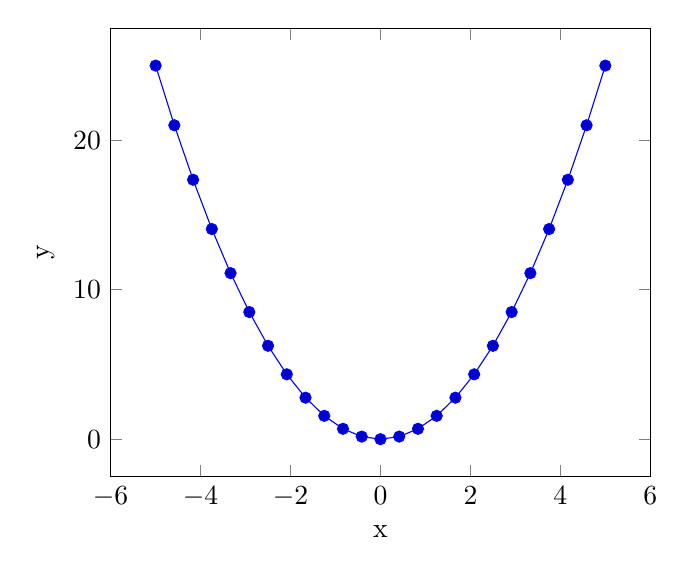
\begin{tikzpicture}% function
	\begin{axis}[xlabel=x, ylabel=y]
	\addplot {x^2};
	\end{axis}
	\end{tikzpicture}
\end{frame}

\begin{frame}[t]{그래프 삽입하기}
	\begin{itemize}
		\item \LaTeX 에서 직접 그래프를 생성하여 삽입하는 방법
		\item \texttt{\tb usepackage\{pgfplots\}}
		\item gnuplot과 유사
		\item \url{http://pgfplots.sourceforge.net/}
	\end{itemize}
	
	\begin{codeblock}{Using pgfplots}
		\texttt{\tb begin\{tikzpicture\}\\
			\hspace{6mm} \tb begin\{axis\}[xlabel=x, ylabel=y]\\
			\hspace{6mm} \tb addplot \{x\textasciicircum 2\};\\
			\hspace{6mm} \tb end\{axis\}\\
			\tb end\{tikzpicture\}}
	\end{codeblock}
	
\end{frame}

\section{Figures}

\begin{frame}[t]{그림 삽입하기}
	\begin{itemize}
		\item \texttt{\tb graphicx} 패키지를 불러오자.
	\end{itemize}
	\begin{codeblock}{graphicx}
		\texttt{\tb usepackage\{graphicx\}}
	\end{codeblock}
	\begin{itemize}
		\item 삽입할 그림은 \texttt{.tex} 파일과 동일한 폴더에 있어야 한다.
		\item 아래 코드를 \texttt{\tb begin\{document\}} 전에 삽입하면 그림을 \texttt{images} 폴더 아래 모을 수 있다.
		
		\begin{codeblock}{graphicspath}
			\texttt{\tb graphicspath\{\{images/\}\}}
		\end{codeblock}
	\end{itemize}
\end{frame}

\begin{frame}[t]{그림 삽입하기}
	
	\begin{figure}[htbp]
		\centering
		
\includegraphics[width=.2\textwidth]{./pictures/GSW_logo.jpg}
		\caption{GSW Logo}
		\label{GSW}
	\end{figure}
	
	\begin{codeblock}{그림 삽입}
		\textbackslash \texttt{begin\{figure\}[htbp]}\\
		\hspace{6mm} \textbackslash \texttt{centering}\\
		\hspace{6mm} \textbackslash \texttt{includegraphics[width=.2\textbackslash textwidth]\{GSW.jpg\}}\\
		\hspace{6mm} \textbackslash \texttt{caption\{GSW Logo\}}\\
		\hspace{6mm} \textbackslash \texttt{label\{GSW\}}\\
		\textbackslash \texttt{end\{figure\}}
	\end{codeblock}
\end{frame}

\begin{frame}[t]{h,t,b,p 옵션}
	'\textbackslash \texttt{begin\{figure\}}' 바로 뒤의 대괄호에 등장하는 옵션에 대해 알아보자.
	\begin{table}
		\centering
		\begin{tabular}{|c|p{0.8\textwidth}|}
			\hline
			h & 개체를 코드의 위치(여기 : \textbf{h}ere)에 놓음 \\
			\hline
			t & 개체를 페이지의 맨 위쪽(\textbf{t}op)에 놓음 \\
			\hline
			b & 개체를 페이지의 맨 아래쪽(\textbf{b}ottom)에 놓음 \\
			\hline
			p & 개체를 특정 페이지(\textbf{p}age)에 놓음. 별다른 설정이 없으면 문서의 맨 뒤. \\
			\hline
			! & \LaTeX 에서 미리 설정해놓은 일부 서식을 무시하고(ex. 텍스트 여백) 놓음\\
			\hline
		\end{tabular}
	\end{table}
\end{frame}

\begin{frame}[t]{Subfigure}
	
	\begin{figure}[h]
		\centering
		\subfigure[h][GSW]{
\includegraphics[width=.2\textwidth]{./pictures/GSW_logo.jpg}}
		\centering
		\subfigure[h][TOR]{
\includegraphics[width=.2\textwidth]{./pictures/Tor_logo.png}}
		\caption{NBA FINAL}
		\label{NBAFINAL}
	\end{figure}
	
\end{frame}

\begin{frame}[t]{Subfigure}
	
	\begin{itemize}
		\item \texttt{subfigure} 패키지를 import 해야 한다.
	\end{itemize}
	
	\hspace{6mm} $\rightarrow$ \textbackslash \texttt{usepackage\{subfigure\}}
	
	\begin{codeblock}{subfigure}
		\textbackslash \texttt{begin\{figure\}[htbp]}\\
		\hspace{6mm} \textbackslash \texttt{centering}\\
		\hspace{6mm} \textbackslash \texttt{subfigure[h][GSW]\{\textbackslash includegraphics\\
			\hspace{6mm} [width=.2\textbackslash textwidth]\{GSW.jpg\}\}}\\
		\hspace{6mm} \textbackslash \texttt{centering}\\
		\hspace{6mm} \textbackslash \texttt{subfigure[h][TOR]\{\textbackslash includegraphics\\
			\hspace{6mm} [width=.2\textbackslash textwidth]\{TOR.jpg\}\}}\\
		\hspace{6mm} \textbackslash \texttt{caption\{NBA FINAL\}}\\
		\hspace{6mm} \textbackslash \texttt{label\{NBAFINAL\}}\\
		\textbackslash \texttt{end\{figure\}}	
	\end{codeblock}
	
\end{frame}

\begin{frame}[t]{pdf 삽입}
	\begin{itemize}
		\item \LaTeX 에서는 pdf를 직접 삽입할 수 있다.
		\item 적당히 잘라 삽입할 수 있다.
	\end{itemize}
	
	\begin{figure}[h]
		\centering
		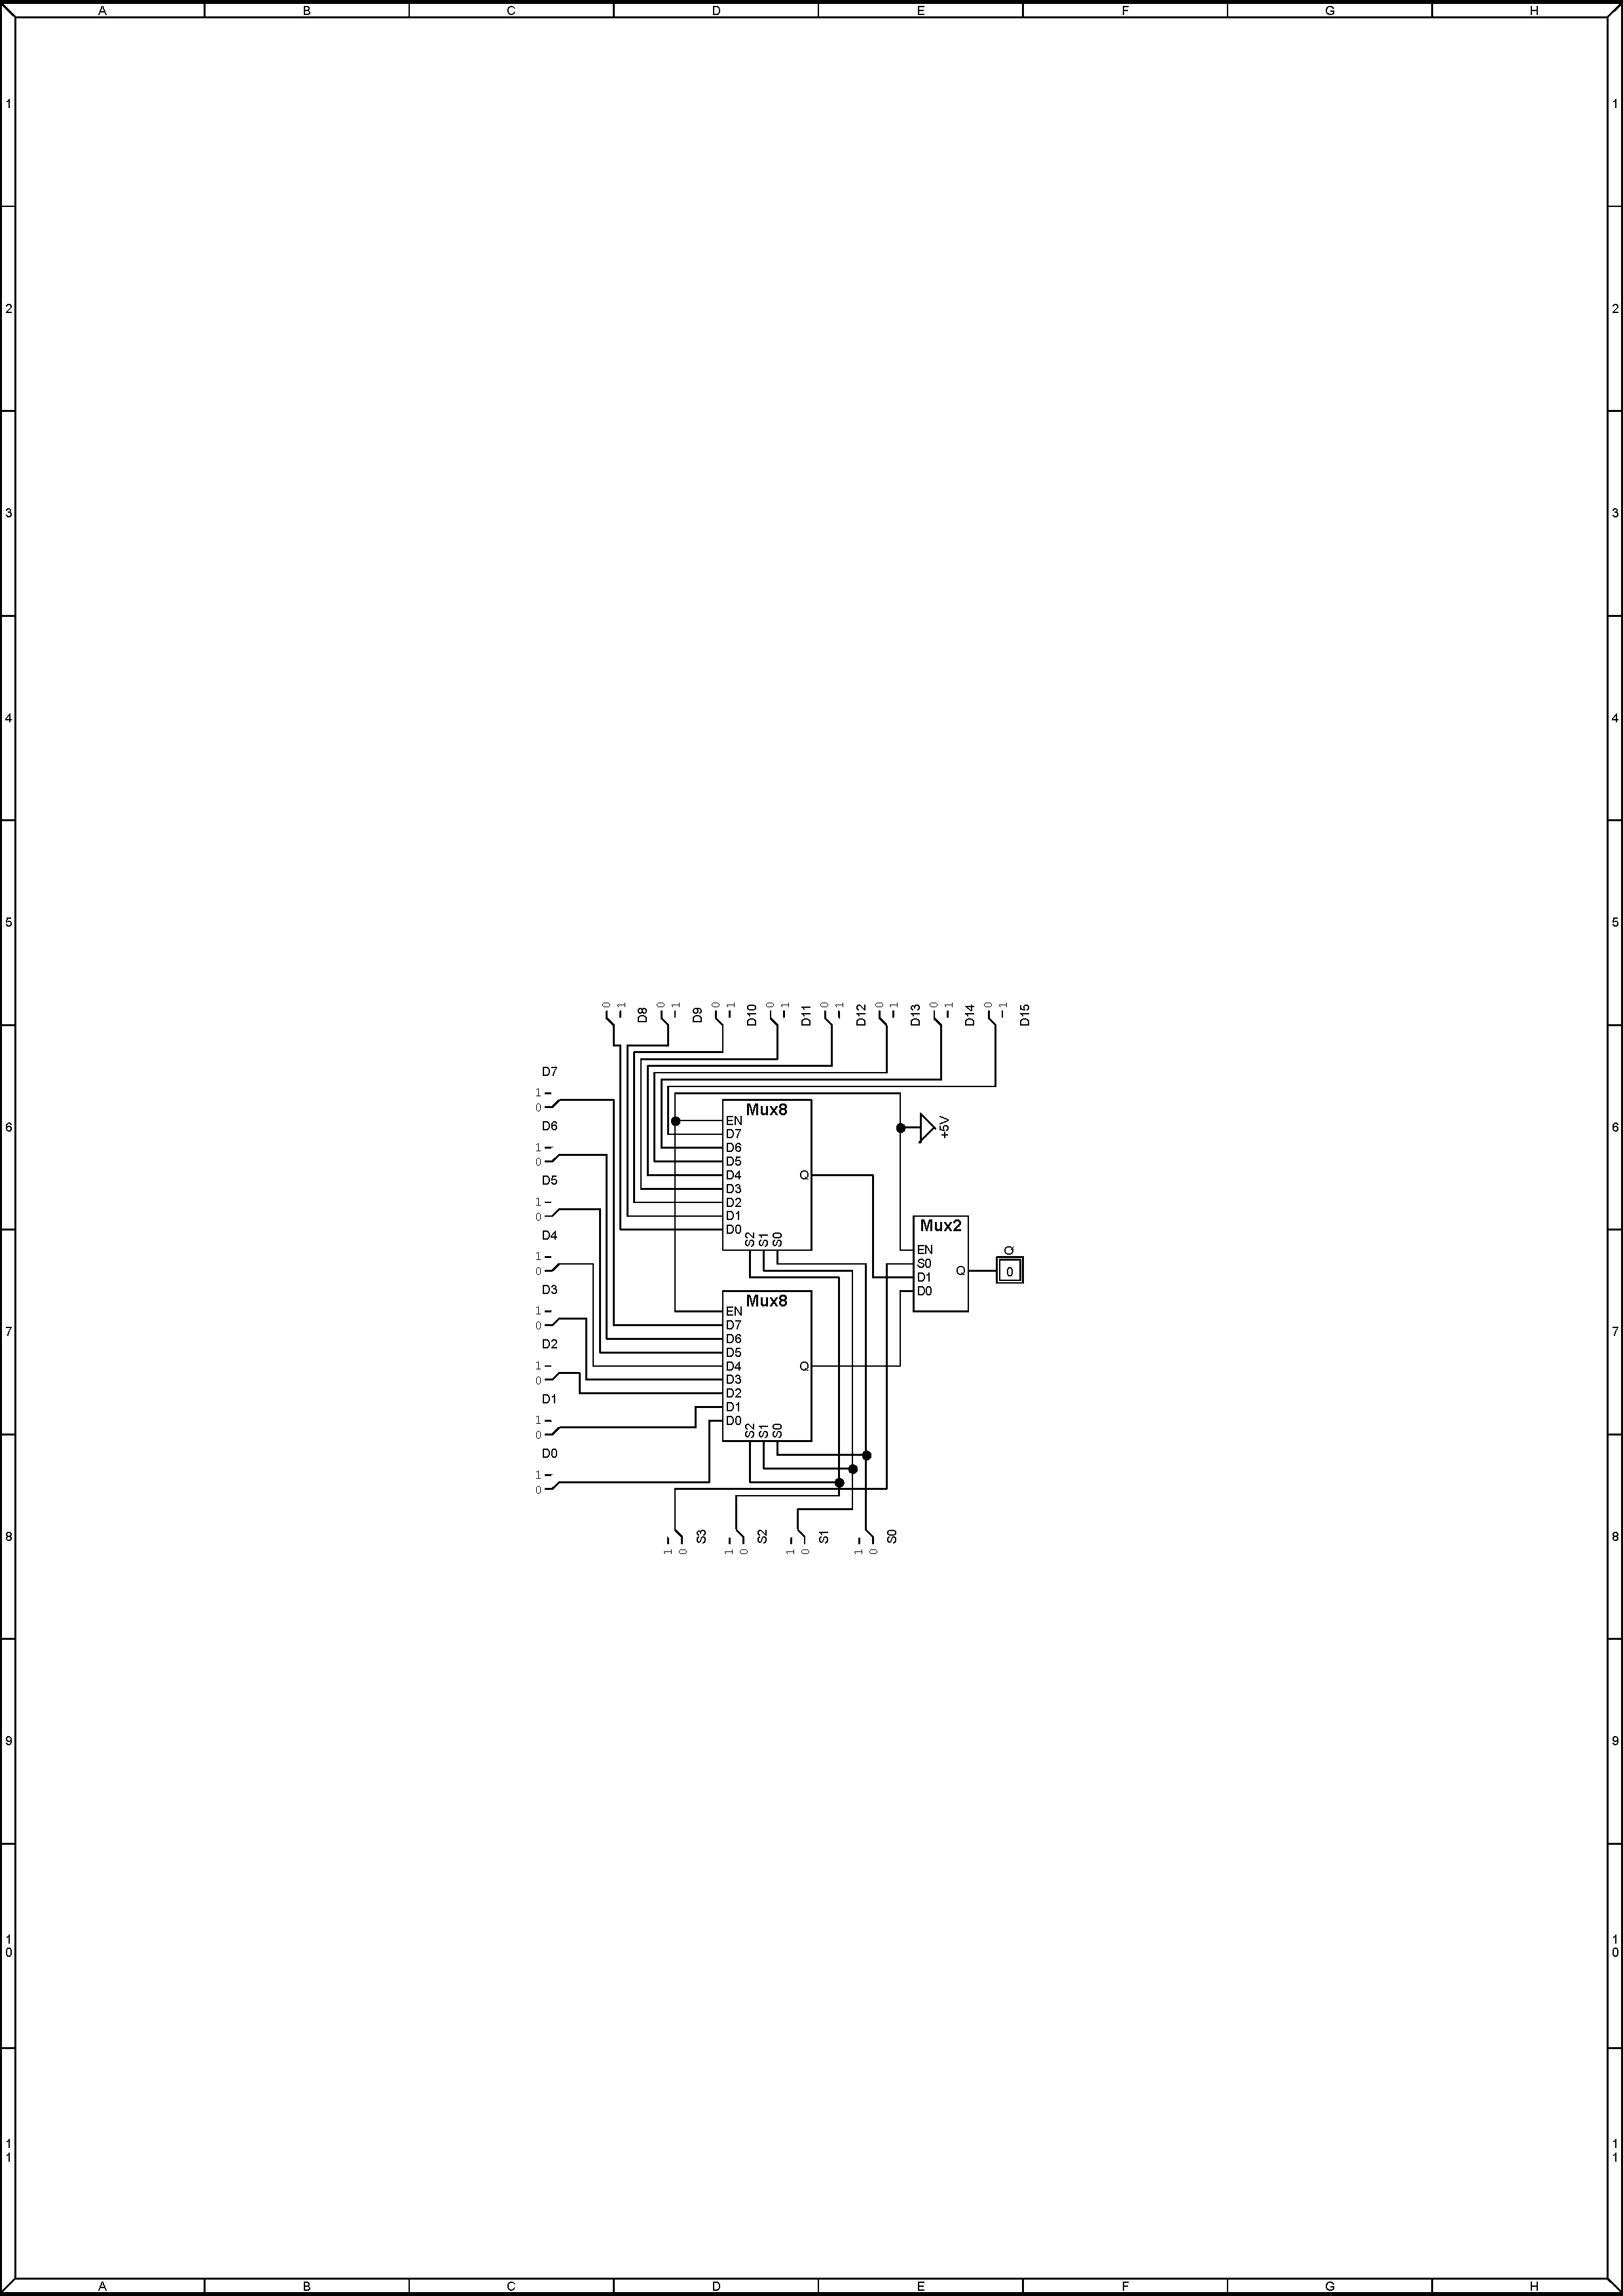
\includegraphics[clip,trim=12cm 19cm 14cm 25cm,width=.6\textwidth]{Example.pdf}
	\end{figure}
	
\end{frame}

\begin{frame}[t]{pdf 삽입}
	\begin{codeblock}{pdf 삽입}
		\texttt{\tb begin\{figure\}[h]\\
			\hspace{6mm} \tb centering\\
			\hspace{6mm} \tb includegraphics[clip,trim=12cm 19cm 14cm 25cm,width=.6\tb textwidth]\{Example.pdf\}\\
			\tb end\{figure\}}
	\end{codeblock}
	
	\begin{itemize}
		\item 그림을 삽입할 때와 비슷하다.
		\item pdf를 crop 할 때는 \texttt{clip, trim}을 사용한다.
		\item 그 뒤의 4개의 수는 각각 left, bottom, right, top의 경계와 pdf의 경계와의 거리를 의미한다.
	\end{itemize}
\end{frame}

\section{Equations}

\begin{frame}[t]{Equations}
	\begin{itemize}
		\item \LaTeX 의 수식에는 두 가지 모드가 있다.
		\begin{itemize}
			\item Inline 모드 : 본문 안에 수식 삽입
			\item Display 모드 : 따로 삽입
		\end{itemize}
	\end{itemize}

	\begin{itemize}
		\item 수식 입력을 위해 \texttt{amsmath} 패키지를 불러오자
	\end{itemize}
	
	\begin{codeblock}{amsmath}
		\tb\texttt{usepackage\{amsmath\}}
	\end{codeblock}
\end{frame}

\begin{frame}[t]{Inline Equations}
	
	\begin{itemize}
		\item 수식을 작성한 뒤 \$ 표시로 감싼다.
	\end{itemize}
	
	\begin{center}
	$ f(x) = \frac{1}{x} $은 반비례 함수이다. \\
	오일러의 공식은 $ e^{i\pi} + 1 = 0 $ 이다. \\
	방정식 $x^{3} = 8$의 실근은 $\sqrt[3]{8} = 2 $ 이다.
	\end{center}

	\begin{codeblock}{수식 작성 예시}
		\texttt{\$ f(x) = \tb frac \{1\}\{x\} \$ 은 반비례 함수이다. } \\
		\texttt{오일러의 공식은 \$ e\^{}\{i\tb pi\} + 1 = 0 \$ 이다. } \\
		\texttt{방정식 \$ x\^{}\{3\} = 8 \$ 의 실근은 \$ \tb sqrt[3]{8} = 2 \$ 이다. } \\
	\end{codeblock}
\end{frame}

\begin{frame}[t]{Inline Equations}
	\begin{itemize}
		\item Inline 모드에서 분수나 대형 기호를 작성할 경우 크기가 줄어들어 보기 싫어진다.
		\item \texttt{\tb displaystyle}을 사용하여 이를 해결할 수 있으나, 이러한 수식은 Display 모드로 작성하는 것이 좋다. 
	\end{itemize}
	
	\begin{center}
		$ f(x) = \frac{1}{x} $ $\rightarrow$ $ \displaystyle f(x) = \frac{1}{x} $
	\end{center}
	
	\begin{codeblock}{displaystyle}
		\texttt{\$ f(x) = \tb frac \{1\}\{x\} \$ } \\
		\texttt{\$ \tb rightarrow \$ } \\ 
		\texttt{\$ \tb displaystyle f(x) = \tb frac \{1\}\{x\} \$ } \\
	\end{codeblock}
	
\end{frame}

\begin{frame}[t]{Displayed Equations}
	\begin{itemize}
		\item \texttt{equation} : 표시형 수식, 번호 있음
		\item \texttt{align} : 수식을 여러 줄에 걸쳐 예쁘게 정리해 줌
		\item \texttt{gather} : 여러 줄로 이루어진 수식을 가운데 정렬
		\item 웬만한 상황에서는 \texttt{align}만 써도 됨
		\vskip 1.5pc
		\item \texttt{\tb label\{\}}을 사용해 라벨을 붙일 수 있고, \texttt{\tb ref\{\}}, \texttt{\tb eqref\{\}}을 이용해 본문에서 참조 가능
		\item 위 환경에서 *을 붙이면 번호가 사라짐
	\end{itemize}
\end{frame}

\begin{frame}[t]{Displayed Equations}
	
	\begin{align}
	e^{i\theta} = \cos{\theta} + i\sin{\theta}
	\label{euler}
	\end{align}
	
	\begin{center}
		오일러의 공식은 \eqref{euler}\과 같다.
	\end{center}
	
	\begin{codeblock}{align + label}
		\texttt{\tb begin\{align\}}\\
		\hspace{6mm} \texttt{e\^{}\{i\tb theta\} = \tb cos\{\tb theta\} + i\tb sin\{\tb theta\}}\\
		\hspace{6mm} \tb \texttt{label\{euler\}} \\
		\texttt{\tb end\{align\}} \\		
		\texttt{오일러의 공식은 \tb eqref\{euler\}\tb 과 같다.}
	\end{codeblock}
	
\end{frame}

\begin{frame}[t]{Displayed Equations}
	
	\begin{itemize}
		\item 라벨 없애기
	\end{itemize}
	
	\begin{align*}
	e^{i\theta} = \cos{\theta} + i\sin{\theta}
	\end{align*}
	
	\begin{codeblock}{align without label}
		\texttt{\tb begin\{align*\}}\\
		\hspace{6mm} \texttt{e\^{}\{i\tb theta\} = \tb cos\{\tb theta\} + i\tb sin\{\tb theta\}}\\
		\texttt{\tb end\{align*\}} \\
	\end{codeblock}

\end{frame}

\begin{frame}[t]{Displayed Equations}
	
	\begin{itemize}
		\item 여러 줄로 된 수식 정렬하기
	\end{itemize}
	\begin{align}
	(x + 1)^2 &= (x + 1)(x + 1)\\
	&= x^2 + x + x + 1\\
	&= x^2 + 2x + 1
	\end{align}
	
	\begin{codeblock}{align}	
		\texttt{\tb begin\{align\}}\\
		\hspace{6mm} \texttt{(x + 1)\^{}2 \&= (x + 1)(x + 1) \tb\tb}\\
		\hspace{6mm} \texttt{\&= x\^{}2 + x + x + 1 \tb\tb}\\
		\hspace{6mm} \texttt{\&= x\^{}2 + 2x + 1}\\
		\texttt{\tb end\{align\}}
	\end{codeblock}
	
\end{frame}

\begin{frame}[t]{Displayed Equations}
	
	\begin{itemize}
		\item \texttt{split}을 사용해 여러 줄로 된 수식 라벨링하기
	\end{itemize}
	\begin{align}
	\begin{split}
	(x + 1)^2 &= (x + 1)(x + 1)\\
	&= x^2 + x + x + 1\\
	&= x^2 + 2x + 1
	\end{split}
	\end{align}
	
	\begin{codeblock}{align + split}	
		\texttt{\tb begin\{align\}}
		\texttt{\tb begin\{split\}}\\
		\hspace{6mm} \texttt{(x + 1)\^{}2 \&= (x + 1)(x + 1) \tb\tb}\\
		\hspace{6mm} \texttt{\&= x\^{}2 + x + x + 1 \tb\tb}\\
		\hspace{6mm} \texttt{\&= x\^{}2 + 2x + 1}\\
		\texttt{\tb end\{split\}}
		\texttt{\tb end\{align\}}
	\end{codeblock}
	
\end{frame}

\begin{frame}[t]{Displayed Equations}
	
	\begin{itemize}
		\item \texttt{multline}으로 긴 수식 작성하기
	\end{itemize}

	\begin{multline}
	f(x + h, y + k) = f(x, y) + h f_{x}(x, y) + k f_{y}(x, y) \\
	+ \frac{1}{2}(h^{2} f_{xx} + 2hk f_{xy} + k^{2} f_{yy})|_{(x, y)} + \cdots \\
	+ \frac{1}{n!}\left(h \frac{\partial}{\partial x} + k \frac{\partial}{\partial y}\right)^{n} f(x, y) + \cdots
	\end{multline}
\end{frame}

\begin{frame}[t]{Equation Tips}
	\begin{itemize}
		\item 큰 괄호 입력하기 (\texttt{\tb left, \tb right})
	\end{itemize}
	\begin{gather}
	\kappa = \frac{1}{|\bold{v}|}\left|\frac{d\bold{T}}{dt}\right| \\
	\int_{1}^{\infty} \frac{1}{x^{2}} dx = \left[-\frac{1}{x}\right]_{1}^{\infty}
	\end{gather}
	\begin{codeblock}{bracket}
	\texttt{\tb begin\{gather\}} \\
	\texttt{\tb kappa  = \tb frac\{1\}\{|\tb bold\{v\}|\} \tb left| \tb frac\{d\tb bold\{T\}\}\{dt\} \tb right|} \\
	\texttt{\tb int\_\{1\}\^{}\{\tb infty\} \tb frac\{1\}\{x\^{}\{2\}\} dx = \tb left[ -\tb frac\{1\}\{x\} \tb right]\_\{1\}\^{}\{\tb infty\}} \\
	\texttt{\tb end\{gather\}}
	\end{codeblock}
\end{frame}

\begin{frame}[t]{Equation Tips}
	\begin{gather}
	\left(\sum_{i=1}^{n} a_{i}b_{i}\right)^{2} \leq \left(\sum_{i=1}^{n}a_{i}^{2} \right) \left(\sum_{i=1}^{n}b_{i}^{2} \right)
	\end{gather}
	\begin{codeblock}{bracket}
		\texttt{\tb begin\{gather\}} \\
		\texttt{\tb left(\tb sum\_\{i=1\}\^{}\{n\} a\_\{i\}b\_\{i\} \tb right)\^{}\{2\} \tb leq \tb left(\tb sum\_\{i=1\}\^{}\{n\} a\_\{i\}\^{}\{2\} \tb right) \tb left(\tb sum\_\{i=1\}\^{}\{n\} b\_\{i\}\^{}\{2\} \tb right) \\ }
		\texttt{\tb end\{gather\}}
	\end{codeblock}
\end{frame}

\begin{frame}[t]{Equation Tips}
	\begin{itemize}
		\item 행렬
	\end{itemize}
	\begin{align}
	\begin{matrix}
	1 & 2 \\ 3 & 4
	\end{matrix} \quad
	\begin{pmatrix}
	1 & 2 \\ 3 & 4
	\end{pmatrix} \quad 
	\begin{bmatrix}
	1 & 2 \\ 3 & 4
	\end{bmatrix}
	\end{align}
	\begin{codeblock}{matrices}
		\texttt{\tb begin\{align\} \\
		\tb begin\{matrix\}
		1 \& 2 \tb \tb 3 \& 4
		\tb end\{matrix\} \tb quad
		\tb begin\{pmatrix\}
		1 \& 2 \tb \tb 3 \& 4
		\tb end\{pmatrix\} \tb quad 
		\tb begin\{bmatrix\}
		1 \& 2 \tb \tb 3 \& 4
		\tb end\{bmatrix\}} \\
		\tb end\{align\}
	\end{codeblock}
\end{frame}

\section{BibTeX}

\begin{frame}[t]{BibTeX}
	\begin{itemize}
		\item 참고문헌 목록을 관리하기 위한 툴
		\item TexStudio에서 새로운 빈 파일을 만들어 작업하고 있는 \texttt{.tex} 파일과 같은 폴더에 \texttt{*.bib}라는 이름으로 저장하자.
	\end{itemize}
\end{frame}

\begin{frame}[t]{BibTeX}
	\begin{itemize}
		\item Google Scholar에서 참고문헌 가져오기
	\end{itemize}
	\begin{figure}
	\centering
	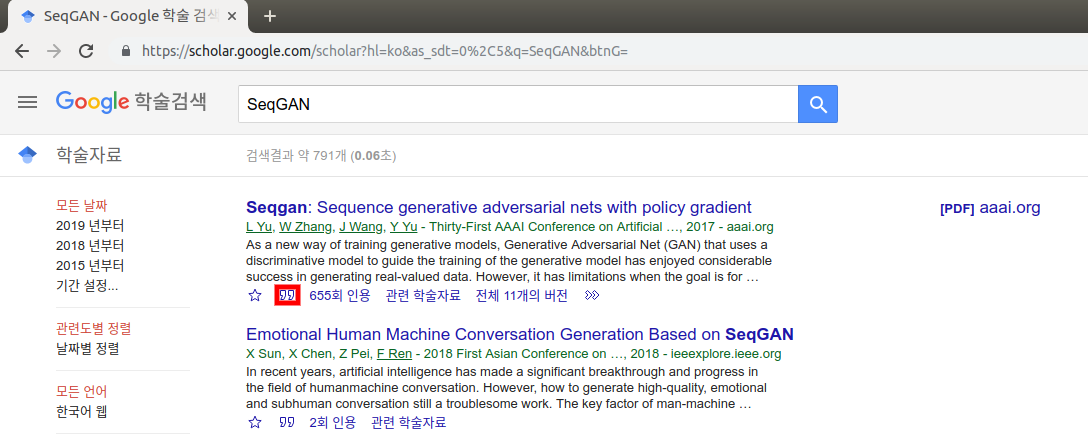
\includegraphics[width=\textwidth]{pictures/scholar1.png}
	\end{figure}
\end{frame}

\begin{frame}[t]{BibTeX}
	\begin{itemize}
		\item Google Scholar에서 참고문헌 가져오기
	\end{itemize}
	\begin{figure}
		\centering
		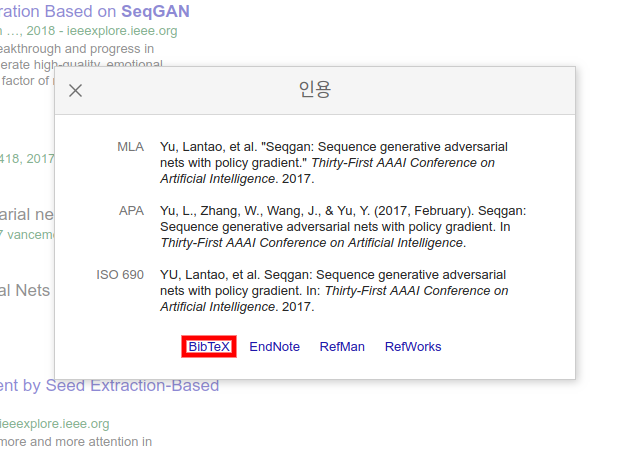
\includegraphics[width=.8\textwidth, clip, trim = 0cm 1cm 0cm 0cm]{pictures/scholar2.png}
	\end{figure}
\end{frame}

\begin{frame}[t]{BibTeX}
	\begin{itemize}
		\item Ctrl-V로 복사 후 \texttt{*.bib} 파일에 붙여넣기
	\end{itemize}
	\begin{figure}
		\centering
		
\includegraphics[width=.7\textwidth, clip, trim = 0cm 1cm 0cm 0cm]{pictures/scholar3.png}
		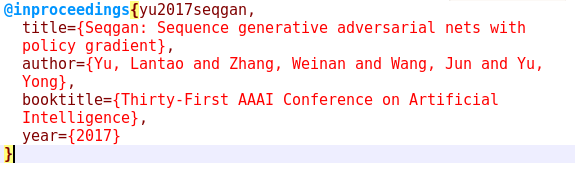
\includegraphics[width=.7\textwidth]{pictures/scholar4.png}
	\end{figure}
\end{frame}

\begin{frame}[t]{BibTeX}
	\begin{itemize}
		\item 본문으로 참고문헌 가져오기
		\item \texttt{\tb bibliographystyle}로 참고문헌 서식 지정
		\item \texttt{\tb bibliography\{\}} 안에 \texttt{*.bib} 파일 이름 넣고 실행
	\end{itemize}
	\begin{figure}
		\centering
		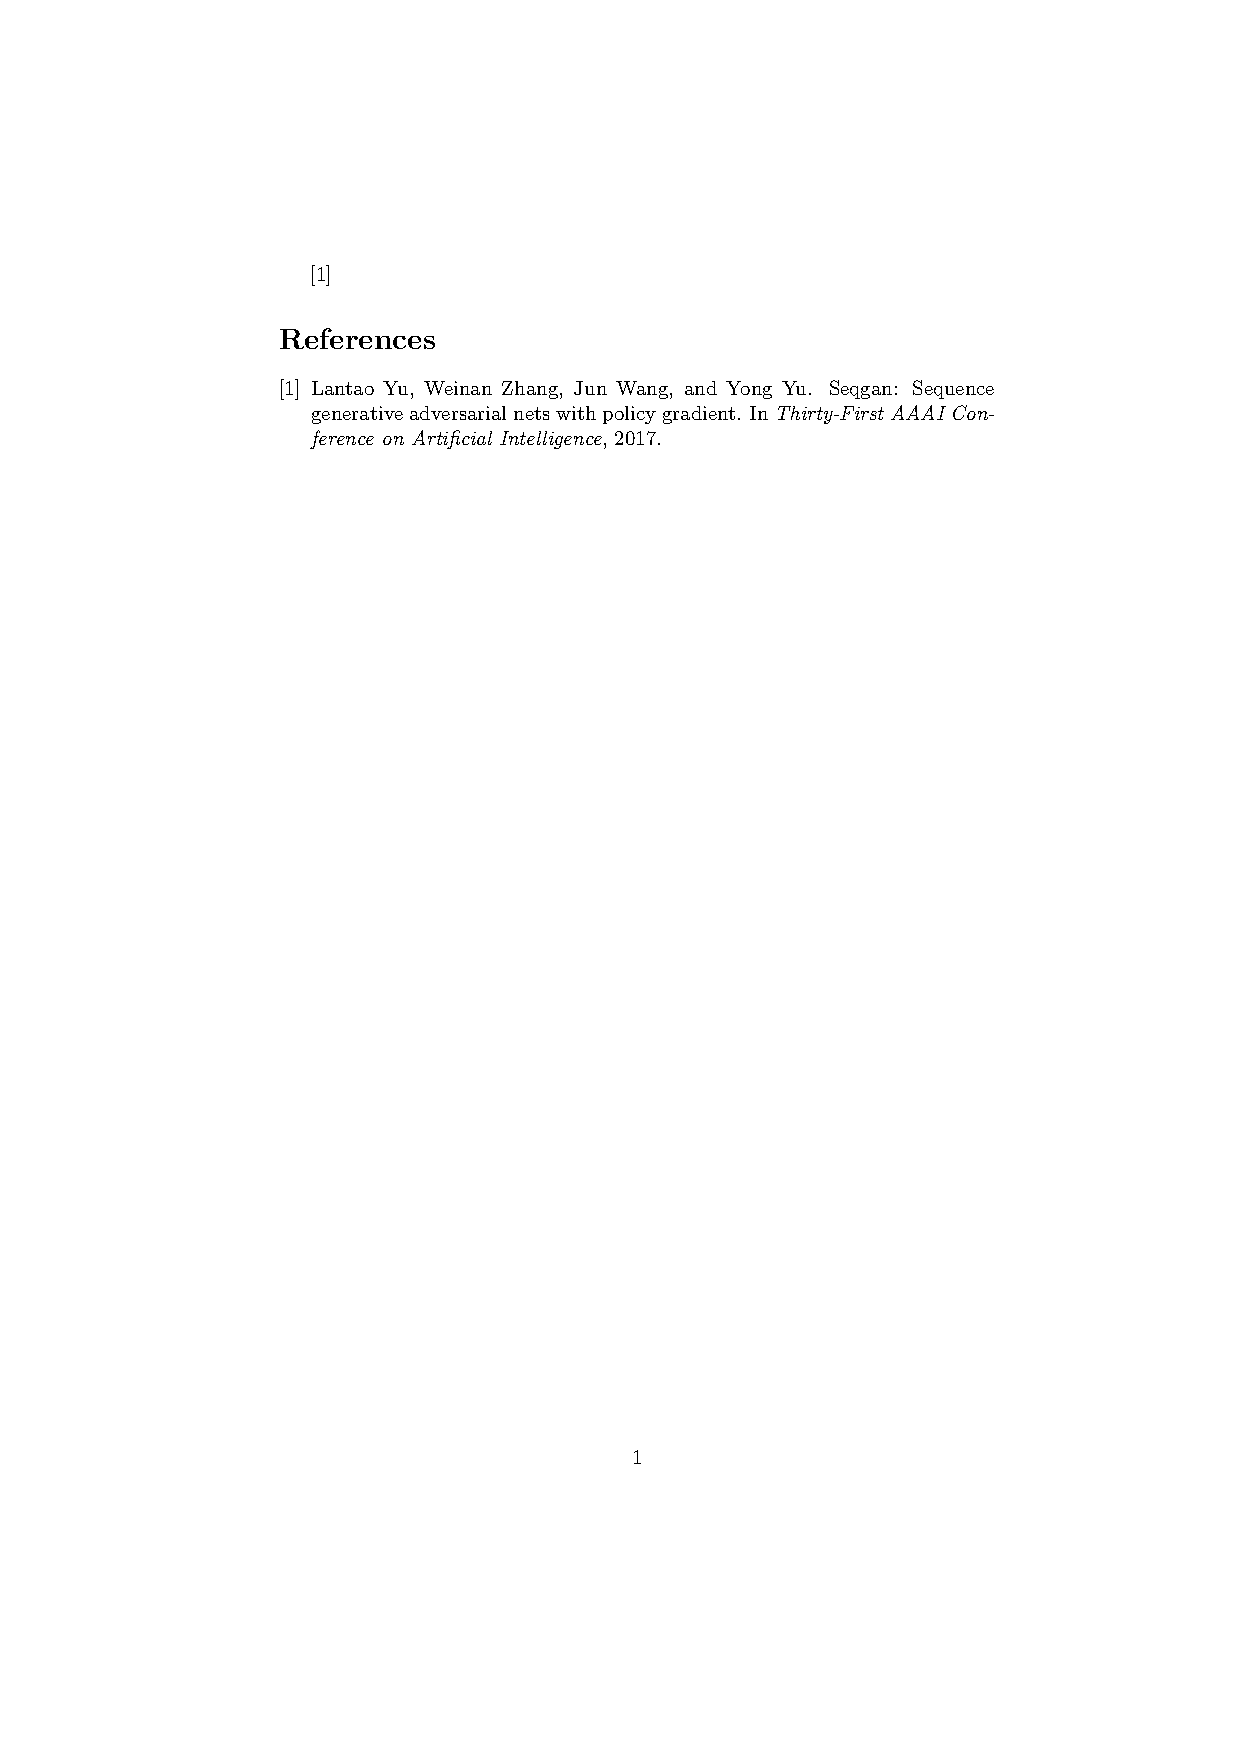
\includegraphics[width=.7\textwidth, clip, trim = 4cm 22cm 4cm 5cm]{ref.pdf}
	\end{figure}
	\begin{codeblock}{BibTeX}
		\texttt{\tb bibliographystyle\{plain\} \\
		\tb bibliography\{references.bib\}}
	\end{codeblock}
\end{frame}

\begin{frame}[t]{BibTeX}
	\begin{itemize}
		\item 본문에서 참고문헌 인용하기
	\end{itemize}
	
	SeqGAN [1]
	
	\begin{codeblock}{BibTeX}
		SeqGAN \texttt{\tb cite\{yu2017seqgan\} }
	\end{codeblock}
\end{frame}

\begin{frame}[t]{경기과학고 \TeX\ 사용자협회}
	\begin{figure}[h]
		\centering
		
\includegraphics[width=\textwidth]{./pictures/homepage.png}
	\end{figure}
\end{frame}

\begin{frame}[t]{경기과학고 \TeX\ 사용자협회}
	\setstretch{1.25}
	\begin{itemize}
		\item 2015.7 : 31기 윤지용의 \TeX\ 졸업논문 공개
		\item 2015.8.2: \url{github.com/gshslatexintro} 개설
		\begin{itemize}
			\item 32기 박승원 - 교우 간 \TeX\ 스터디 활동을 위해 개설
		\end{itemize}
		\item 2015.12 :
	\end{itemize}
	\begin{quote}
		"\TeX 사용에 대한 진입 장벽을 없애고, \\
		\TeX 을 사용한다면 누구나 쓸 수 있는 \\
		각종 양식 파일을 공유하고 공동 편집하자!"
	\end{quote}
	\vspace{-.5cm}
	\begin{flushright}
		--- 32기 협회 일동
	\end{flushright}
	$ \rightarrow $ 텍 입문서 제작, 텍 워크샵 진행, 각종 텍 예제 및 양식 제작/배포 등\ldots
\end{frame}

\begin{frame}[t]{경기과학고 \TeX\ 사용자협회}
	\begin{itemize}
		\item 각종 양식 및 입문서, 예시작 온라인 제공
		\begin{itemize}
			\item 주소 : \url{latex.gs.hs.kr}
			\item 지금 보고 있는 이 자료도 홈페이지에서 다운 가능!
		\end{itemize}
		\item 양식
		\begin{itemize}
			\item R\&E, 졸업논문, 휴먼테크, beamer 등
		\end{itemize}
		\item 예시(예제)
		\begin{itemize}
			\item 예제 코드를 보면서 \TeX\ 배우기 (굉장히 중요)
		\end{itemize}
		\vspace{1cm}
		\item {\scriptsize \textbf{다운로드 방법} : \url{latex.gs.hs.kr} - 다운로드 - `다운로드 페이지 링크'}
	\end{itemize}
	
\end{frame}

\begin{frame}[t]{구인 광고}
	\begin{itemize}
		\item 본 협회의 활동에 참여하고 싶다면,
		\begin{itemize}
			\item GitHub에 가입한 뒤
			\item username을 서울 선생님께 발송.
			\item \url{github.com/gshslatexintro} 멤버에 추가
			\item 선생님들께서도 참여 가능합니다.
		\end{itemize}
		\vskip 1pc
		\item 저희선배가 그랬듯이, 저희가 그랬듯이, 양식 제작 등의 활동을 하며 텍을 공부해볼 수 있을 것입니다. 절호의 기회를 놓치지 마세요!
		\begin{itemize}
			\item 5代 회장 및 개발진, 웹마스터 모집.
		\end{itemize}
	\end{itemize}
	
\end{frame}

\end{document}